\textbf{Research Plan and Methodology}\\

We describe seven major tasks to be completed over two years. The project time schedule for each task is shown in the gantt chart.
%This proposed study will have two main goals, with
%sub-tasks corresponding to the six objectives specified in Part II 1(b).
%The project will be completed over two years as shown in the project time schedule
%in Figure 1.

Task B to D correspond to the three main steps of our method for generating an animation from a given sketch and a corresponding video (Figure 2): feature points extraction and alignment, motion extraction from the video and video-to-sketch motion transfer.
{The alignment step extracts good feature points from both the video and the sketch and compute their one-to-one correspondence. The motion step tracks the feature points in the video frames guided by a structure graph, which is useful for detecting and {estimating the positions} of the drifting points. Finally, the extracted motion is transfered to the sketch via a stroke-preserving deformation method to produce the final animation.}

%\begin{figure}
%	\centering
%	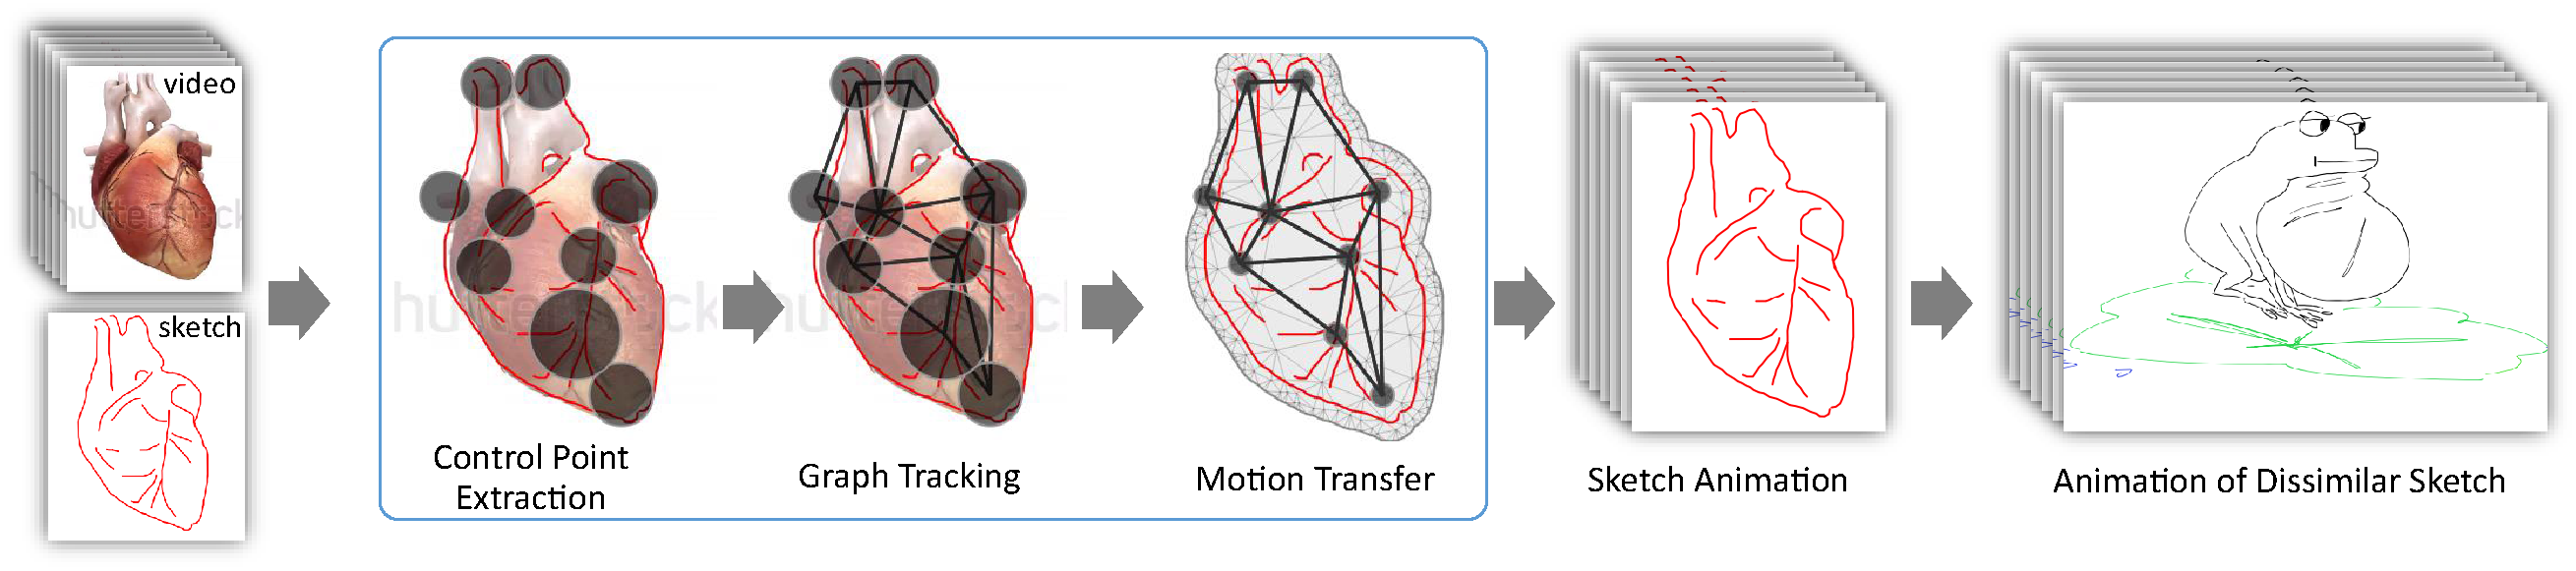
\includegraphics[width=0.85\linewidth]{images/overview}
%	\caption{}
%	\label{fig:overview}
%\end{figure}
%
%\begin{figure}
%	\centering
%	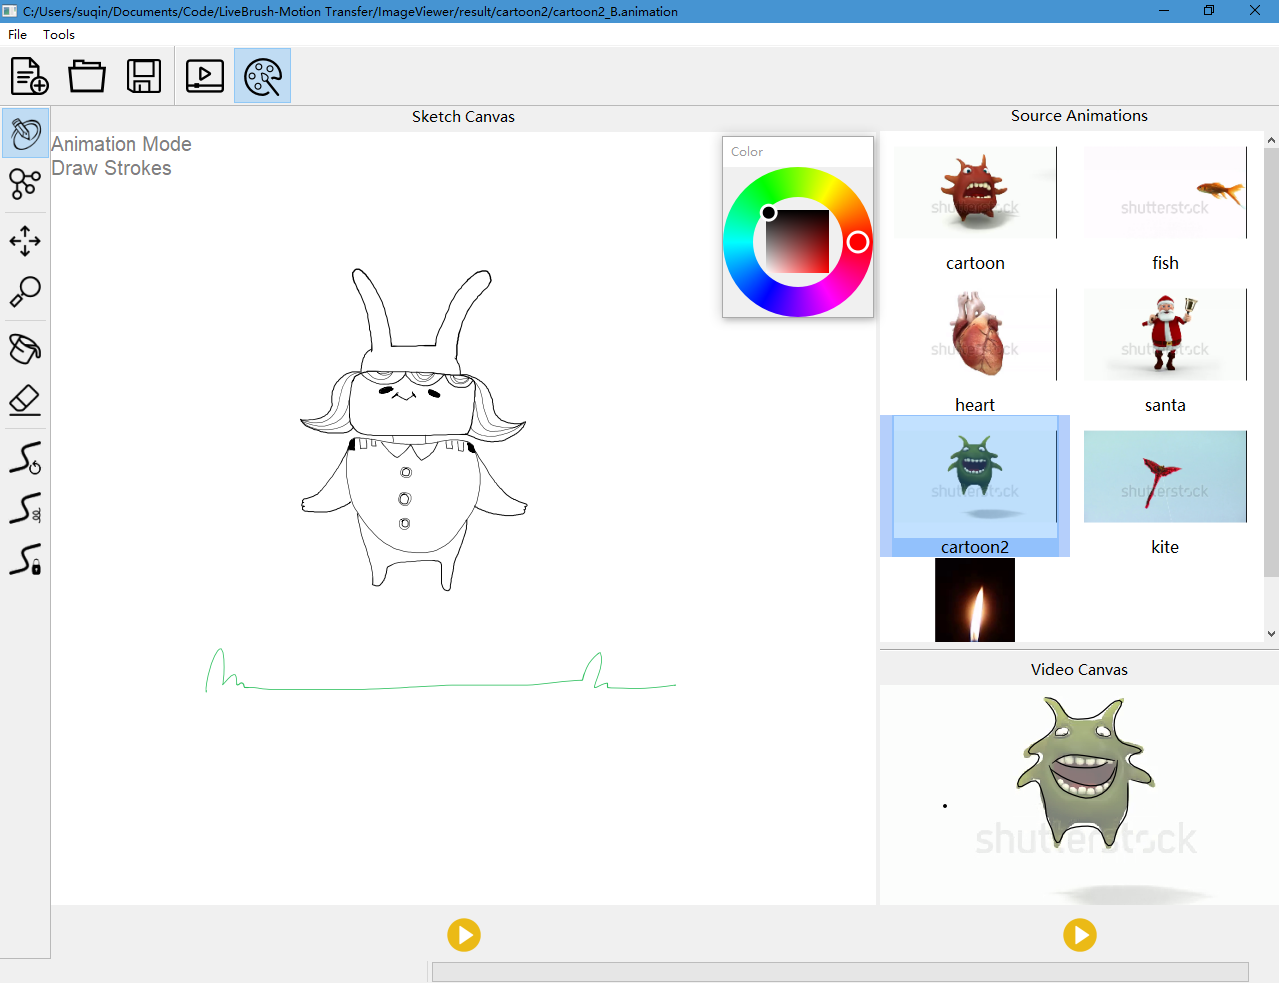
\includegraphics[width=0.85\linewidth]{images/ui}
%	\caption{}
%	\label{fig:ui}
%\end{figure}

\textbf{Task A: Interface Design}

%Our system, Live Sketch, will aim at providing novice users with an easy way to animate their drawings by existing videos. The input is a sketch and a video.
%The user draws the sketch and the system animates the sketch using the motion extracted from the video automatically or with few user interactions for aligning the sketch with the object in the video.
%
The user interface (Figure 1) of Live Sketch will include a tool bar, a video window, a sketch window and a playback controller. 
The {\em video window} and the {\em sketch window} will show the corresponding video and sketch animation frame at a selected time position, respectively. 
Users may sketch a free-hand drawing in the sketch window or sketch over an image in the video window aided by an image tracking tool
like EZ-Sketching~\cite{EZSketching:2014}. 
The {\em tool bar} will list all the tools for animation creation. 
The {\em playback controller} will contain buttons for controlling the playback of the video and 
the animation.
After an animation is generated, the user can select one frame of the animation for preview by moving the slider or browsing the 
frame list in the {\em playback controller} area.

\textbf{Task B: Feature Extraction and Alignment}

Finding a correspondence between the video and the sketch is a challenging problem, because the former is a collection of meaningless pixels while the latter is vector graphics which is more abstract. The goal here is to extract feature points that are good to track from the video, which will also match well the user's interest in animating the sketch.
We will first extract feature points from the first video frame by a scale-irrelevant corner detection method~\cite{grauman:2011}.
Some of these extracted features may have no corresponding part in the sketch, i.e., they may not be of the user's interest (e.g., gray circles in Figure 3a), and vice versa.

%In addition, the sketch and the video frame may not align well (see the two examples in Figure 1 and Figure 3a,b). 
%\ca{filtering solves alignment problem?} Therefore, we need to filter out such feature outliers and find the correspondence between these remaining good features in the video and the sketch \cfm{this sentence lumps the above two problems together.}

{We extract feature points from the sketch by the approach of finding the local maxima of a feature map (Figure 3b). We construct the feature map for the vector graphics sketch by assigning the feature value of 1 at the endpoint of each stroke and assign the curvature value at each inner stroke point, normalized to $[0,1]$, and then apply Gaussian smoothing. The feature points are then identified by finding the local maximum within a certain radius, which is dependent on the stroke thickness.  Note that using an image corner detection method on a rasterized sketch image may not work because crossings in the sketch will be incorrectly identified as corners, \ca{such as two crossing arms or self-crossing strokes}. 
} 

After obtaining the feature points from the first frame of the video and feature points from the sketch,
we will find the optimal bipartite matching by a non-rigid ICP point set matching method~\cite{Chui2003114}.
% \ca{because} it aims to find a global non-rigid matching for all points.
All unmatched feature points are then omitted. Subsequent steps will use the 
established one-to-one correspondence.
%Matchings with large matching energy are also removed from the results \ca{since the matching is}. 
%\ca{All the remaining matchings} provides a good overall alignment, which satisfies both the user's interest in the sketch while being good tracking features in the video.


%$ \mathbf{P} = \{P_i | P_i = (\mathbf{x}_i, r_i)\} $ 

In some cases, {the user may need to delete some extracted features to simplify the animation}, or add more features to include more animation details. 
There may also exist too large structural dissimilarity between the sketch and the video for determining a desirable feature correspondence automatically (see Figure 3c,d).
Therefore, the user interface will also allow users to manually add or remove feature points or edit their positions or correspondences.
Note that even though these {refining} manual operations may take some time, the feature extraction and alignment process is done for only one frame and does not require any animation experience. The next two steps are efficient and fully automatic. 
%contrast with time-consuming keyframe-based methods. 


%\begin{figure}
%	\centering
%	\includegraphics[width=0.85\linewidth]{images/alignment}
%	\caption{Two examples}
%	\label{fig:alignment}
%\end{figure}


\textbf{Task C: Motion Extraction}

The goal of the motion extraction step is to extract a robust motion trajectory for each matched video feature point. However, since {the animation result} is very sensitive to motion consistency of adjacent points, it will be necessary to preserve the object structure {among the features during tracking}.

%We will propose a structure detection and correction two-step method for motion extraction.  During tracking, drifting points are detected and their positions will be predicted later by considering their spatial and temporal neighborhood.

% defined over the extracted tracking points.
Since the sketch possesses more structure information of the user's interest, we construct the object structure based 
on the sketch. 
Denote the structure graph as $ \mathcal{G} = (\mathcal{V}, \mathcal{E}) $, where $ \mathcal{V} $ is the set of feature points of the video and 
$ \mathcal{E} $ is a subset of edges of Delaunay triangulation of points in $ \mathcal{V} $. 
Specifically, we need to exclude certain edges of the Delaunay triangulation, in particular, those that crosses concave shape boundaries (e.g., the edge connecting the 4th and 8th points in Figure 5b).
% as such an edge would limit the moving of the fire or distort the static candle.}
We determine $\mathcal{E}$ by first computing the outline of the sketch using an active contour method, designate the interior region as the sketch mask and eliminate all edges that lie partially outside the sketch mask. 
%We compute a sketch mask which defines the region the sketch covers. 
%We let $ \mathcal{E} $ be all the edges that lie completely inside the sketch mask.

%If two points are connected by the sketch lines or the inter-sketch parts of the path is small, they would be connected in the structure graph. 

We will develop a structure-preserving tracking method that solves an energy optimization problem comprising
two energy terms:
appearance energy $ E_t $, which measures the appearance dissimilarity between a point and its candidate tracking point,
%  is computed for each tracking feature point using existing tracking methods such as Struck~\cite{6126251}
and structure energy $ E_s $, which measures the structure deformation error relative to {the} initial structure.
%To solve this optimization problem, we propose the following method. 
For each feature point in the first frame, we will determine a candidate set of tracked points {in the new frame} (the circles in Figure 5c,d, e). 
Denote the candidate set of the $i$th point as $ \mathbf{C}_i  = \{C_{ij}\}$, $j = 1, 2, \ldots, n_i $,  with their appearance energy in ascending order, where the $ j $th candidate $ C_{ij} = (\mathbf{x}_{ij}, r_{ij}) $ contains its position $ \mathbf{x}_{ij} $ and size $ r_{ij} $ in pixels.
The appearance energy $ E_t $ 
can be computed using a state-of-art object tracking method such as Struck~\cite{6126251}. 
Specifically, the appearance dissimilarity is measured based on the positiveness of a given sample after running a SVM classication over all samples.

We first simply choose the candidate \ca{with minimal appearance energy} as the tracking result of each feature point. This may cause structure distortion. We therefore will propose a two-step method that first detects the drifting points with the help of the structure graph and correct their positions later.  
Denote {a candidate combination as $ \mathbf{K} = (C_{1j_1}, C_{2j_2},\ldots, C_{nj_n}) $ representing a specific possible combination of chosen candidates of features. 
%{Let the structure energy measures the distortion of the graph relative to its original position.}
We compute the local structure energy for the $ j $th candidate $ C_{ij} $ of $ i $th feature point given a candidate combination $ \mathbf{K} $ as follows:
\begin{align}\label{eq:structure_energy}
E_s(C_{ij}|\mathbf{K}) = \sum_{(i, k) \in \mathcal{E}} \|(\mathbf{x}_{ij} -  \mathbf{x}_{kj_k}) - (\mathbf{x}^1_{i} -  \mathbf{x}^1_{k}) \|^2_2,
\end{align}
where $ \mathbf{x}^1_i $ denotes the initial position in the first frame, initialized in the feature extraction step, and 
$\mathbf{x}^1_k$ denotes a neighbor.  This energy measures the edge-length difference relative to the initial position.
We will first find the feature point that has the largest structure energy in its local subgraph (consisting of the point and its {one-ring} neighbors). Then its candidate whose structure energy is the minimal and lower than a threshold $ \eta $ will be chosen. If no such candidate exists, the point will be flagged as drifting and {its position} will be determined by considering its spatial and temporal neighborhood in the motion transfer step. Repeat this step until all the feature points have chosen their best candidates or have been flagged as drifting. 
%Because tracking each feature independently may lead to undesired structure distortion, we preserved several candidates for each point from the tracking samples of small appearance energy.  So this could be formulated as a energy minimization problem over all candidate combinations in $ \mathcal{K} = \{\mathbf{K} | \mathbf{K} = (C_{1j_1}, C_{2j_2},\ldots, C_{nj_n})\} $
%
%\begin{align}\label{eq:motion_min}
%\mathbf{K}^* = \arg\min_{\mathbf{K} \in \mathcal{K}} \sum_{i} E(C_{ij_i}|\mathbf{K})
%= {\arg}\min_{\mathbf{K} \in \mathcal{K}} \sum_{i} E_t(C_{ij_i}|\mathbf{K}) + \alpha E_s(C_{ij_i}|\mathbf{K})
%\end{align}
%
%, where $ E_s = \sum_{(i, j) \in \mathcal{E}} \Delta d$ is measured by the edge length and angle difference regarding to initial object position.
%
%However, 1) it requires searching exponentially many configurations; 2) some candidates may break the structure even if they may have small appearance energy. Therefore, we will propose a method based on graph matching that could avoid the two problems(Algorithm~\ref{alg:motion_extraction}).  
%Algorithm 1~\ref{alg:motion_extraction} summarizes the algorithm. 
Algorithm 1 summarizes the algorithm. 

%\begin{comment}
%\begin{algorithm}
%	\caption{Motion Extraction}\label{euclid}
%	%\label{alg:motion_extraction}
%	
%	\begin{algorithmic}[1]
%		\Require Video $ V $, Feature points $ \mathbf{P}^1 = \{P^1_i | P^1_i = (\mathbf{x}^1_i, r^1_i)\} $ at the first frame.
%		
%		\Ensure Structure-preserving tracking result $ \mathbf{P}^t = \{P^t_i | P^t_i = (\mathbf{x}^t_i, r^t_i)\} $ for each frame.
%		
%		\State Construct the structure graph $ \mathcal{G} = (\mathcal{V}, \mathcal{E}) $.
%		
%		\For {$ t = 2 : m $}
%		\LongState{Extract the candidate set for each feature point: $ \mathbf{C}_i  = \{C_{ij}\} $ where $ C_{ij} =
%			(\mathbf{x}_{ij}, r_{ij}), j = 1, 2, \ldots, n_i$}.
%		
%		%\State Initialization: $ \mathbf{P}^t \gets (C_{11}, C_{21}, \ldots, c_{n1}) $
%		
%		\LongState {Find the best candidate configuration $ \mathbf{K}^* = (C^*_1,\ldots,C^*_n) $ by \ca{selecting} the best candidate for each feature point that minimizes the structure energy (Eq.~\ref{eq:structure_energy}). The drifting feature points $  \mathbf{S} = \{i | E(C^*_i|\mathbf{K}^*) > \eta \} $ are also detected. $ \forall i \notin \mathbf{S}, P^t_i \gets C^*_i. $}
%		\LongState {Predict the drifting points' positions $ \{ P^t_i | i \in \mathbf{S}\} $ from spatial neighbors in motion transfer step.} 
%		\EndFor
%		
%		\State {Refine} the positions of drifting points $ \{ P^t_i | i \in \mathbf{S}\} $ according to their global motion trajectory.
%		
%		\State \Return $ \{\mathbf{P}^t\} $.
%		%		\While {true}
%		%		\State $ i^* \gets \max_i E_t(C^*_i) + \alpha E_s(C^*-C^*_i) $
%		%		\State $ j^* \gets \min_j E_t(c_{i^*j}) + \alpha E_s(C^*-C^*_{i^*} + c_{i^*j}) $
%		%		
%		%		\EndWhile
%		%		
%		%		\State $\textit{stringlen} \gets \text{length of }\textit{string}$
%		%		\State $i \gets \textit{patlen}$
%		%		\If {$i > \textit{stringlen}$} \Return false
%		%		\EndIf
%		%		\State $j \gets \textit{patlen}$
%		%		\If {$\textit{string}(i) = \textit{path}(j)$}
%		%		\State $j \gets j-1$.
%		%		\State $i \gets i-1$.
%		%		\State \textbf{goto} \emph{loop}.
%		%		\State \textbf{close};
%		%		\EndIf
%		%		\State $i \gets i+\max(\textit{delta}_1(\textit{string}(i)),\textit{delta}_2(j))$.
%		%		\State \textbf{goto} \emph{top}.
%		%		\State \Return $ C $
%		
%	\end{algorithmic}
%\end{algorithm}
%\end{comment}

%\begin{figure}[t]
%	\centering
%	\includegraphics[width = 0.95\linewidth]{algorithm}
%	\caption{}
%	\label{fig:mesh}	
%\end{figure}



%Existing related work that try to resolve this problem, such as single or object tracking using geometric model~\cite{Martinez20083682,Artner20111969,6243144,6934993,zhang2013structure}, which could tolerant some drifting problems or matching errors. However, these methods usually used a global optimization for all parts/objects, which may lead to either a global drifting problem when using strong structure constraint, or structure distortion at some parts/object because of using strong appearance trackers. 
%Our method is different with structure-preserving previous single/multiple object tracking methods. 
Previous single object tracking methods~\cite{Martinez:2008,Artner:2011,Cehovin:2013,Cai:2014} {often utilize weak local features of sampled patches to track a single window. The window position is determined from all patches through a voting or statistical method. Even though the weak features bring inaccuracy to tracking of each small patch, such inaccuracy is not critical when tracking only one window. Our application, however, is sensitive to structure distortion. We believe the detection and correction two-step method can avoid large distortion.} 

%The structures used in existing multiple object tracking methods\cite{Zhang:2013} is different with ours. 
%Existing multi-object tracking methods are typically more flexible and do not have as strong structure \ca{among features} as \ca{single object} in our application. Furthermore, most of them are one-step tracking methods that do not correct positions when drifting occurs \ref{XXX}.

%methods~\cite{Martinez:2008,Artner:2011,Cehovin:2013,Cai:2014,Zhang:2013}, including the structure preserved multi-object tracking methods, our method is a detection and correction two-step method. It insures to avoid sketch distortion after the motion is transfered. 


\textbf{Task D: Motion Transfer}

The motion transfer step aims to apply the extracted motion to the sketch, respecting the established correspondence. For this purpose, we will devise a variant of the as-rigid-as-possible (ARAP) mesh deformation method~\cite{Igarashi:2005}.
We will first generate a mesh by triangulating the sketch mask region obtained in Task B.
%To generate the mesh for sketch deformation, we triangulate the contour that is obtained using active contour method for the sketch image.
The sketch feature points, excluding the drifting points,  serve as control points for deforming the sketch. 
%The sketch can then be animated by manipulating the sketch feature points as handles for deformation.
However, the original ARAP mesh deformation only aims to keep the rigidity of the mesh triangles (see Figure 4a) and
thus cannot preserve the stroke shape.
A direct solution might be to add a shape constraint for each stroke in the energy minimization formulation, and express each stroke point as an interpolation of neighboring mesh vertices. However, at areas with higher stroke density, preservation of the stroke shapes would require re-triangulation to obtain higher triangle density. To avoid this problem, we will add a new triangle set that serves to preserve the stroke shapes and another set of 
triangles that propagates the original mesh deformation as a soft force to the sketch.
%Denote the feature positions of the $ t $th and $ (t + 1) $th frame as $ \mathbf{p}^t = \{p^t_{i}\} $ and $ \mathbf{p}^{t+1} = \{p^{t + 1}_{i}\} $.
Specifically, we will modify the original mesh (gray in Figure 4a) $ \mathcal{M}_0 = (\mathcal{V}_0, \mathcal{T}_0) $ by adding all the sampled stroke points $ \mathcal{V}_s $ and constructing two new triangle sets $ \mathcal{T}_s $ and $ \mathcal{T}_l $, i.e.,
$ \mathcal{M} = (\mathcal{V}_0 \cup \mathcal{V}_s, \mathcal{E}_0 \cup \mathcal{T}_s \cup \mathcal{T}_l) $. 
The \textit{sketch triangle set} $\mathcal{T}_s $ is constructed by connecting every three successive points on each stroke (purple triangles in Figure 4a).
The \textit{link triangle} set $\mathcal{T}_l $ is constructed by connecting each sketch point with the three vertices of the triangle on which it lies
(cyan triangles in Figure 4a).

%\begin{figure}[t]
%	\centering
%	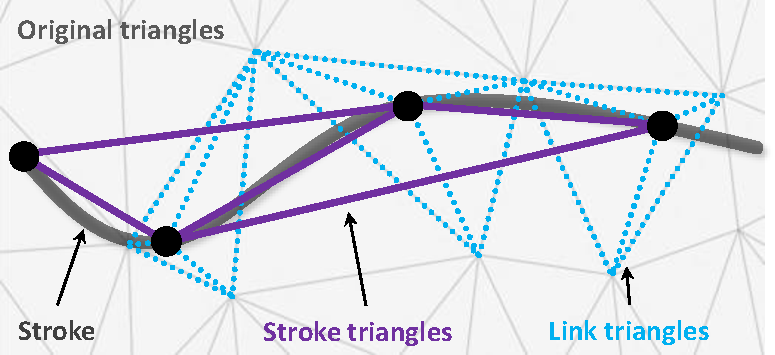
\includegraphics[width = 0.95\linewidth]{images/mesh}
%	\caption{Reconstructed mesh for stroke-preserving ARAP deformation.}
%	
%	\label{fig:mesh}	
%\end{figure}

We will formulate the stroke-preserving ARAP deformation as the following energy minimization problem: 
\begin{align}
\min_\mathcal{M} \ E_0 + E_{link} + \beta E_{sketch},
\end{align}
where $ E_0 $ is the deformation energy of the original mesh $ \mathcal{M}_0 $ relative to the original mesh position, and $ E_{link} $ and $ E_{sketch} $ represent the deformation energy of the newly constructed triangle sets $\mathcal{T}_l $ and $\mathcal{T}_s $, respectively. Minimizing $ E_{sketch} $ keeps the shape of the strokes while minimizing $ E_{link} $ transfers the deformation of the original mesh to the strokes. The weight of $ E_{link} $ is set to 1 so that the link triangles will be as rigid as the original mesh, while the weight of the stroke triangles, $ \beta $, is set large ($ > $ 1) so that the shape of the strokes is preserved. 
%
Figure 4 shows an expected result of our proposed stroke-preserving ARAP deformation method.

The drifting points are not used as control points of deformation because their positions are unreliable. Their positions are interpolated from their spatial and temporal neighbors after deformation. Since interpolated positions from the deformed mesh may not be consistent with their temporal neighborhood, which may lead to the {shuffling problem at these drifting frame positions}, we will therefore also smooth the {temporal} trajectories of these drifting points. 

\textbf{Task E: Evaluation}

%Our system aims at providing the user with an easy way to add 3D strokes to an existing shape for communicating conceptual design ideas. Strokes drawn by a user over an existing 3D shape are generally of two types. The first type lie on an existing surface. The 3D information for such a stroke can be determined easily by projection onto the surface. The second type of strokes are drawn to specify a non-existent part of the shape, indicating how the original shape is to be modified. Determining the 3D information for this type of stroke is nontrivial. Our system focuses on providing an interface to draw sketch strokes of the second type.

We will conduct a user study to evaluate our system. The user study will consist of two parts. In User Study I, a number of participants will be invited to use both our system and an existing state-of-the-art keyframe method such as Adobe Animator to create two animations for every given pair of sketch and video. 
To evaluate the efficiency of our system, 
%In this experiment, the participants will be asked to create a sketch animation to a given video. 
we will compare the completion time and the number of operations which include the sketching operations and the editing operations. 
The participants will also be asked to answer a questionaire on the usability of our system. 

The sketch animations created using the two methods will then be evaluated by a different group of participants in User Study II.
We will ask the participants to score each sketch animation created in User Study I on aesthetics, completeness, etc. 


\textbf{Task F: Applications}

We will extend the basic \textit{Live Sketch} to two applications.
%	\textbf{Many-to-one motion transfer}
	Segmenting a character into meaningful parts or layers and animating them separately is common in animation creation. Similarly, our system will also allow transferring motions from multiple videos to different parts of a single sketch. Independent motion transfer for each part will lead to spatial inconsistency, which can be solved by existing motion retargeting method such as AniMesh~\cite{Jin:2015}.
	Another way to increase the usability of motions is to transfer motions to a sketch in different temporal intervals.  We will need to address the issue of smooth transitions between motions.
Note that in such scenarios the number of control points used in the two motions may be different but the original mesh is the same as
the two motions are transferred to the same sketch. 
%the two sets of control points positions between the two control point sets at the transition position may not be well aligned and may locate at different parts of the sketch. 
A possible solution to attain smooth transition from motion A to motion B is as follows (see Figure 6). We first compute the position of each control point of A on B's deformed mesh by mesh interpolation. Next we can find a new motion trajectory for each point of motion A during B's time interval. A smooth transition trajectory can easily be found between the two trajectories by Hermite 
interpolation.
%by Laplacian smoothing after connecting them. 
%Similarly, we can obtain a smooth transition trajectory for each control point of motion B. Therefore, the animation can be transited smoothly based on the transition trajectories.
	
	Interactive illustrations can provide a more playful or informative experience~\cite{Kazi:2014b}. We will also extend our \textit{Live Sketch} tool to achieve dynamic interactive animations. Users can interact with the animation to control its playback direction, speed of playing and locally deform near a dragged point. 
	We will provide a user interface that when the user drags one part of the sketch, the animation will be played forward or backward according to the drag direction with respect to the nearest motion trajectory. The speed of playing will depends on the cursor speed.  The point on the sketch where it is being dragged will be deformed such that it stays attached to the cursor. This can be achieved by applying a sketch deformation method described in Task D, where the drag point is treated as an additional control point.
% (user is also required to give another static point). 
	Different dynamic motion constraints can also be specified to different parts, for example, producing the effect of magnifying the motion of certain parts while suppressing the motion of the other parts. 
Furthermore, dynamic dragging constraints can also be applied to simulate effects such as flowers being blown by wind.  

	%It also allow user to add an external force like wind with dynamic direction and speed.
%We provide a user interface that when user drag some part of the sketch, the animation would be played adaptively and dynamically and also respect to user's dragging position. The animation speed and direction can be computed by the dragging speed and direction. To make sure that the dragging part is always attached to the cursor, a sketch deformation is applied to the deformed sketch using the method in Task D, where the dragging point is treated as the control point (user is also required to give another static point). Furthermore, our system can also produce dynamic animation when user specifies dynamic dragging constraints such as the wind, or highlights the motion of some parts by magnifying its motion and reducing others'.


\textbf{Task G: Extensions}

Our tool aims to animate a sketch using the same motion of the object in the video, it thus will look as real as in the video. Since the users might want to produce a stylized animation, we will provide post-animation stylization tools, such as using animation filters~\cite{Wang:2006}, applying the 12 animation principles~\cite{Kazi:2016}, and adding animation looping.

%{The methodology described above focuses on motion transfer for a single object.} An extracted motion can also be re-used and transferred to multiple objects.  In that case, motion re-targetting is necessary. 

%We will also investigate creation of sketch animations containing numerous objects. For this purpose, we will need to design and implement a new user interface that can combine the results of several animation results of our method into one scene.

Sketching on touch-based devices is direct and natural. Hence,
implementing Live Sketch on devices like iPad and iPhone will be highly desirable.  This will require redesigning the user interface to improve user experience on sketching and interactions, such as integrating multitouch features and stylus pen.

%In our system, we require only coplanar strokes be drawn in each step. This setting ensures that our system is able to generate the expected 3D sketch with only simple interaction. However, this restriction may hinder the user during drawing. The ultimate goal of allowing the user to draw strokes on arbitrary planes or surfaces in any order is too difficult. Instead, we will further investigate how to make our system more general by introducing other type of constraints besides the coplanar constraint for drawing strokes, constraining the current set of drawn curves to be on a curved surface, or to be symmetric. 
%%\ca{Similar to the current algorithm, we will borrow the geometry information to constrain the drawn curves. Specifically, 
%If the matched sharp edges are on a common curved surface that is extracted from the shape, the surface is a potential canvas. If the drawn strokes are self-symmetrical after an affine transformation, the canvases that realize this transformation might be desirable ones. When the user draws a set of strokes, it is unknown which constraint should be used. A possible solution will be to traverse all the constraints and generate all possible candidate 3D strokes which will be ranked using the same criteria described before.

%An issue to solve then would be how does the system automatically recognize what type of constraint to enforce on the drawn strokes. \ca{Possible solutions? curved surface derived from the given shape}

%Man-made shape is the main focus of our system. It is because designing man-made shapes is more common than organic shapes. 
%For example, the user may want to modify the design of an existing furniture model, or change the appearance of a building model. When designing a 3D scene, the models in this scene are mostly man-made. In our system, we will mainly focus on the following information.

